\chapter{Monitorowanie klienta mobilnego}
\label{chap:Wymagania}

\section[Monitorowanie rozproszone][Monitorowanie rozproszone klientów
statycznych]{Monitorowanie rozproszone klientów statycznych}

Firmy działające obecnie na rynku posiadają bardzo rozbudowaną
infrastruktę informatyczna. Od bardzo wielu lat działy odpowiedzialne
za utrzymanie infrastruktury informatycznej prowadzą ciągły monitoring
zarówno urządzeń sieciowych jak i~serwerów oraz stacji roboczych
użytkowników. Bardzo wiele firm posiada również specjalistyczne
urządzenia, które również muszą być podłączone do sieci i~monitorowane
w~celu zapewnienia ciągłości procesów biznesowych danej
firmy. Powyższe urządzenia rozumiane są jako klienty
statyczne. Urządzenia tego typu zazwyczaj pracują nieprzerwanie lub
w~dobrze zdefiniowanych przedziałach czasowych i~posiadają dobrze
zdefiniowaną hierarchię. Wzajemne relacje pomiędzy tymi urządzeniami
wynikają w~dużej mierze z~struktury sieci lecz mogą również wynikać
z~roli jaką pełnią one w~danej organizacji. Dzięki monitorowaniu
wszystkich urządzeń w~danej sieci systemy monitorujące są w~stanie
wspierać administratora wskazując z~bardzo dużym prawdopodobieństwem
miejsce wystąpienia awarii.

Sieć w~dużej firmie rzadko stanowi jedną całość. Zazwyczaj są to
segmenty sieci oddzielone zaporami lub w~ogóle oddzielnie sieci LAN
lub VLAN. Taka separacja urządzeń pozwala na zwiększenie poziomu
bezpieczeństwa, lecz jednocześnie utrudnia monitorowanie całej
infrastruktury. Aby umożliwić monitorowanie całej sieci firmowej
wykorzystywane jest monitorowanie rozproszone. Można wyróżnić dwie
podstawowe konfiguracje monitorowania rozproszonego:

\begin{itemize}
\item Monitorowanie pasywne: Istnieje jedna, centralna instancja jądra
  monitorującego, do którego przesyłane są wyniki sprawdzeń
  poszczególnych usług. Każde urządzemoe samo monitoruje swoje usługi
  i~zgłasza rezultaty.
\item Wieloinstancyjny system monitorujący: Istnieje wiele instancji
  jądra monitorującego. Typowo, każda wydzielona część sieci posiada
  swoją instancję. Każda instancja może posiadać zarówno usługi
  monitorowane aktywnie jak i~pasywnie. Wyniki sprawdzeń przesyłane są
  następnie do jednej wybranej instancji, która gromadzi wszystkie
  dane.
\end{itemize}

\begin{figure}[h]
\label{fig:PorPasIRozp}
  \caption{Monitoring pasywny oraz rozproszony. Kolor czerwony -
    monitorowanie aktywne, niebieski - monitorowanie pasywne, czarny -
    komunikacja wewnętrzna systemu.}
\makebox[\textwidth]{%
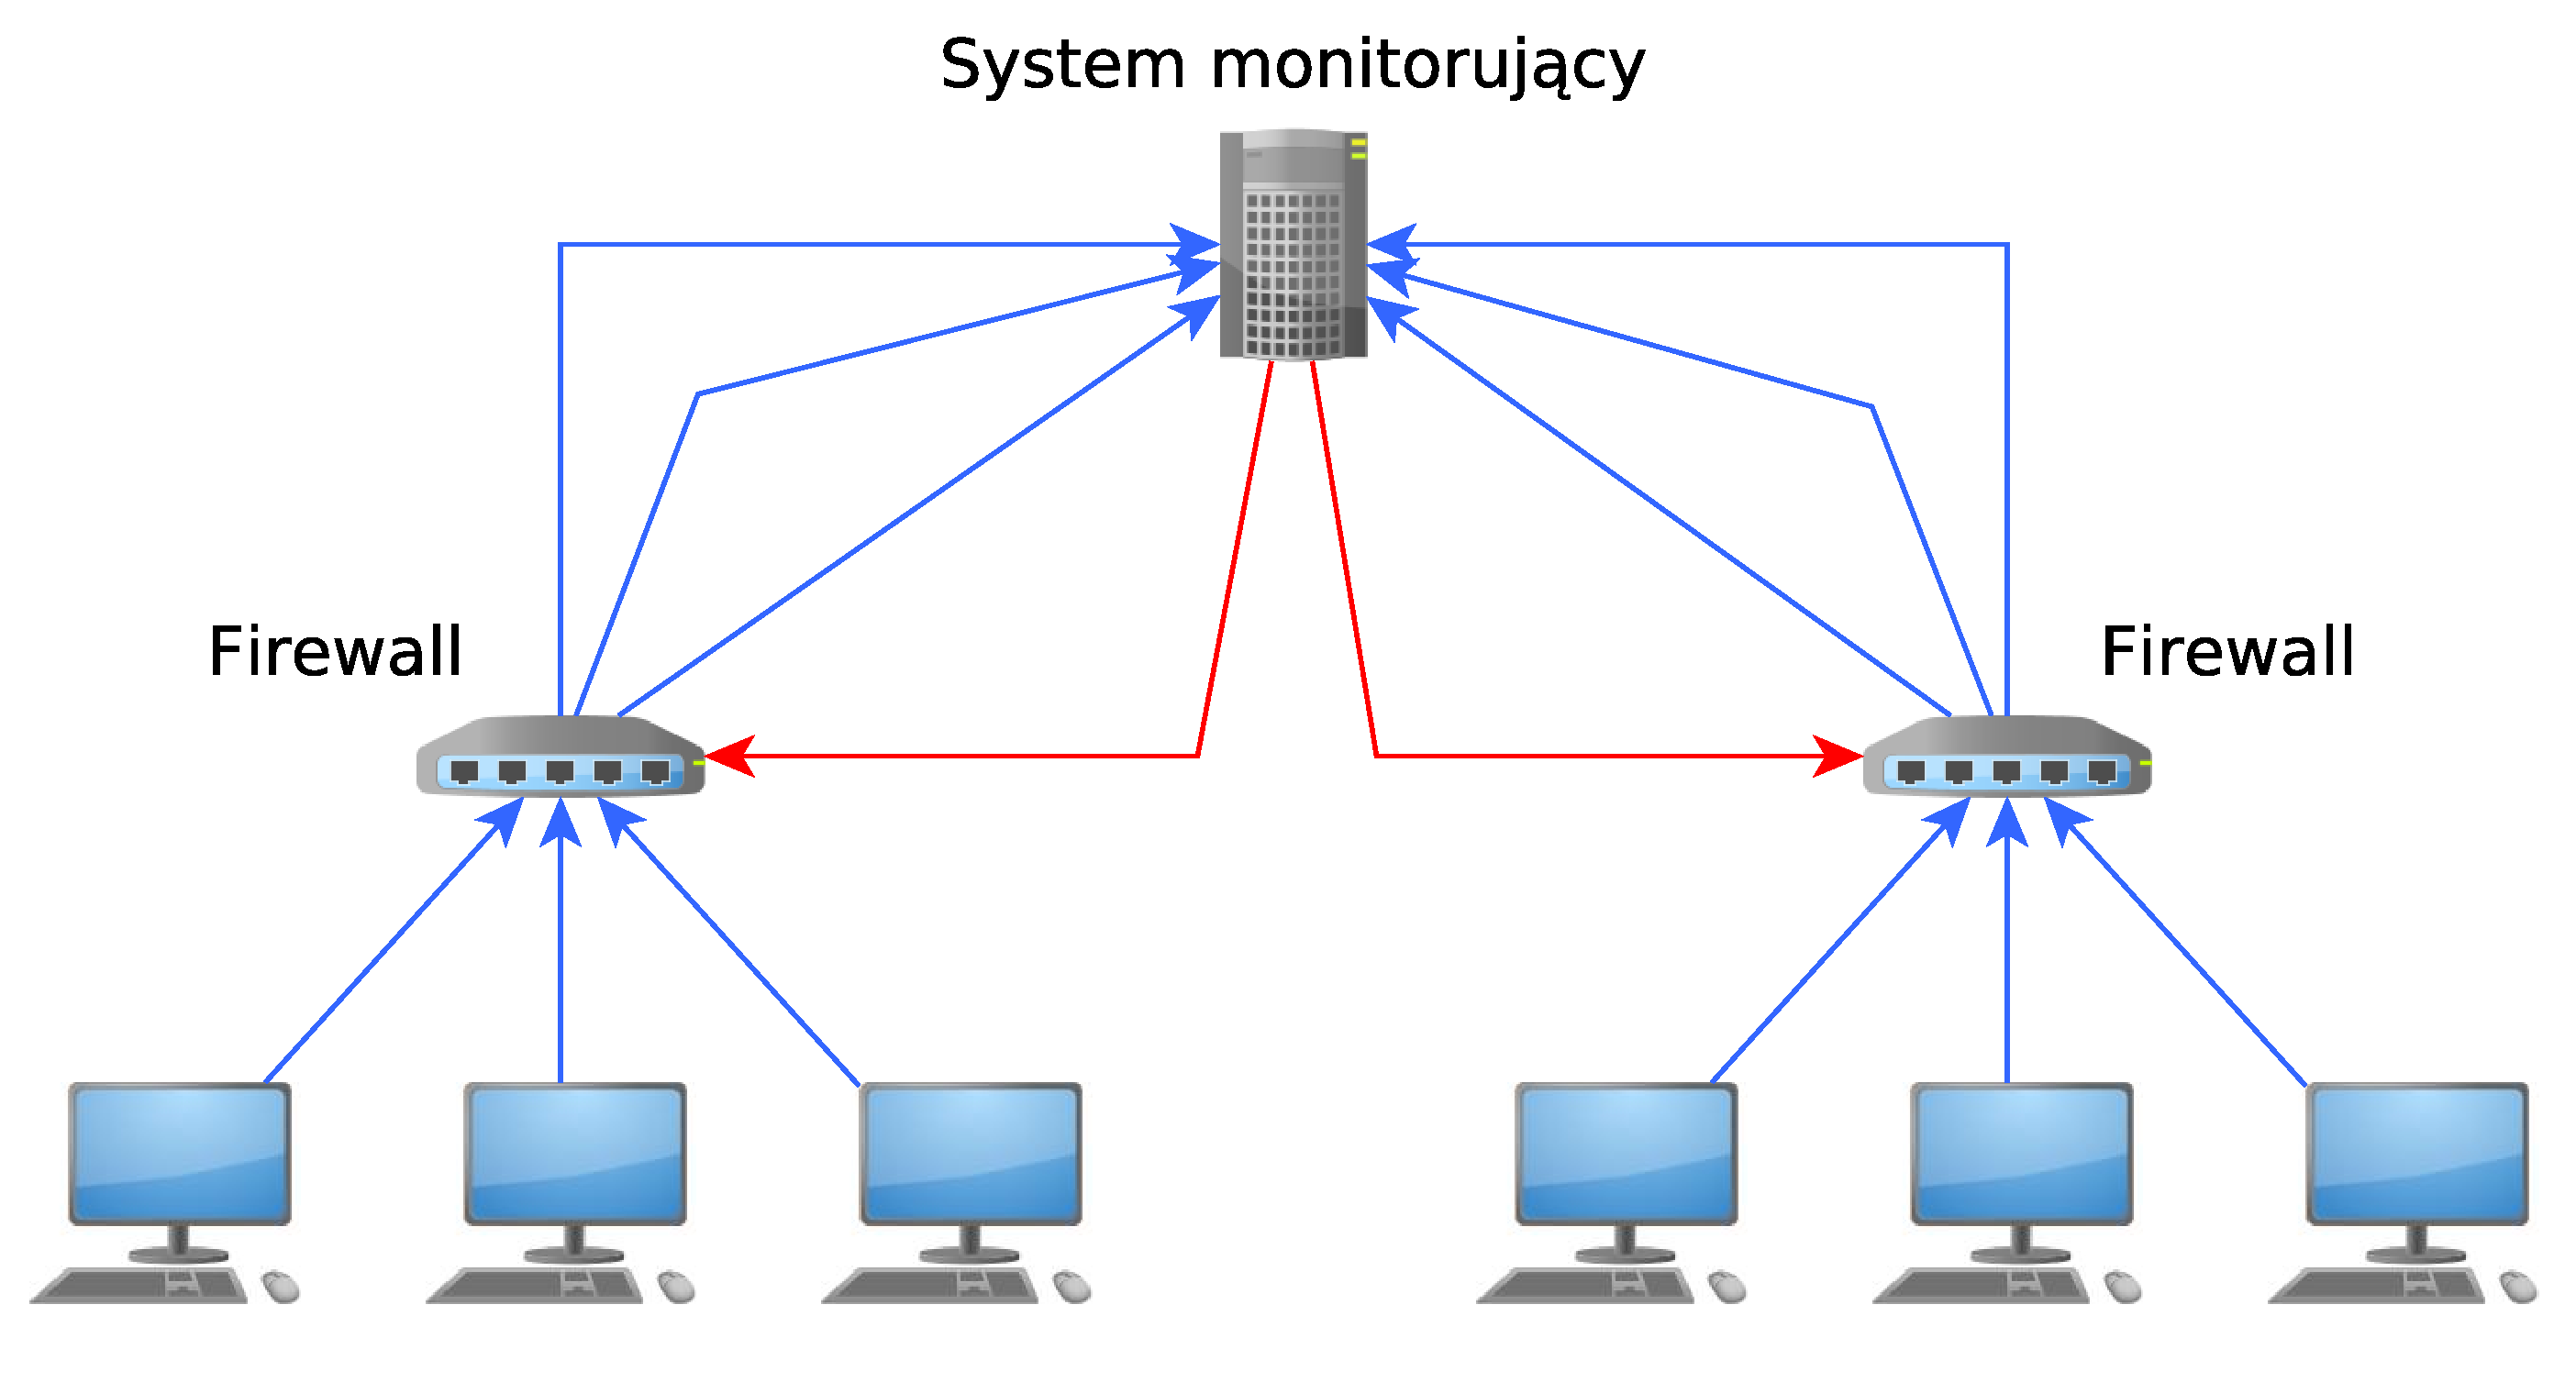
\includegraphics[width=0.49\textwidth]{img/pasywne}
\hfill    
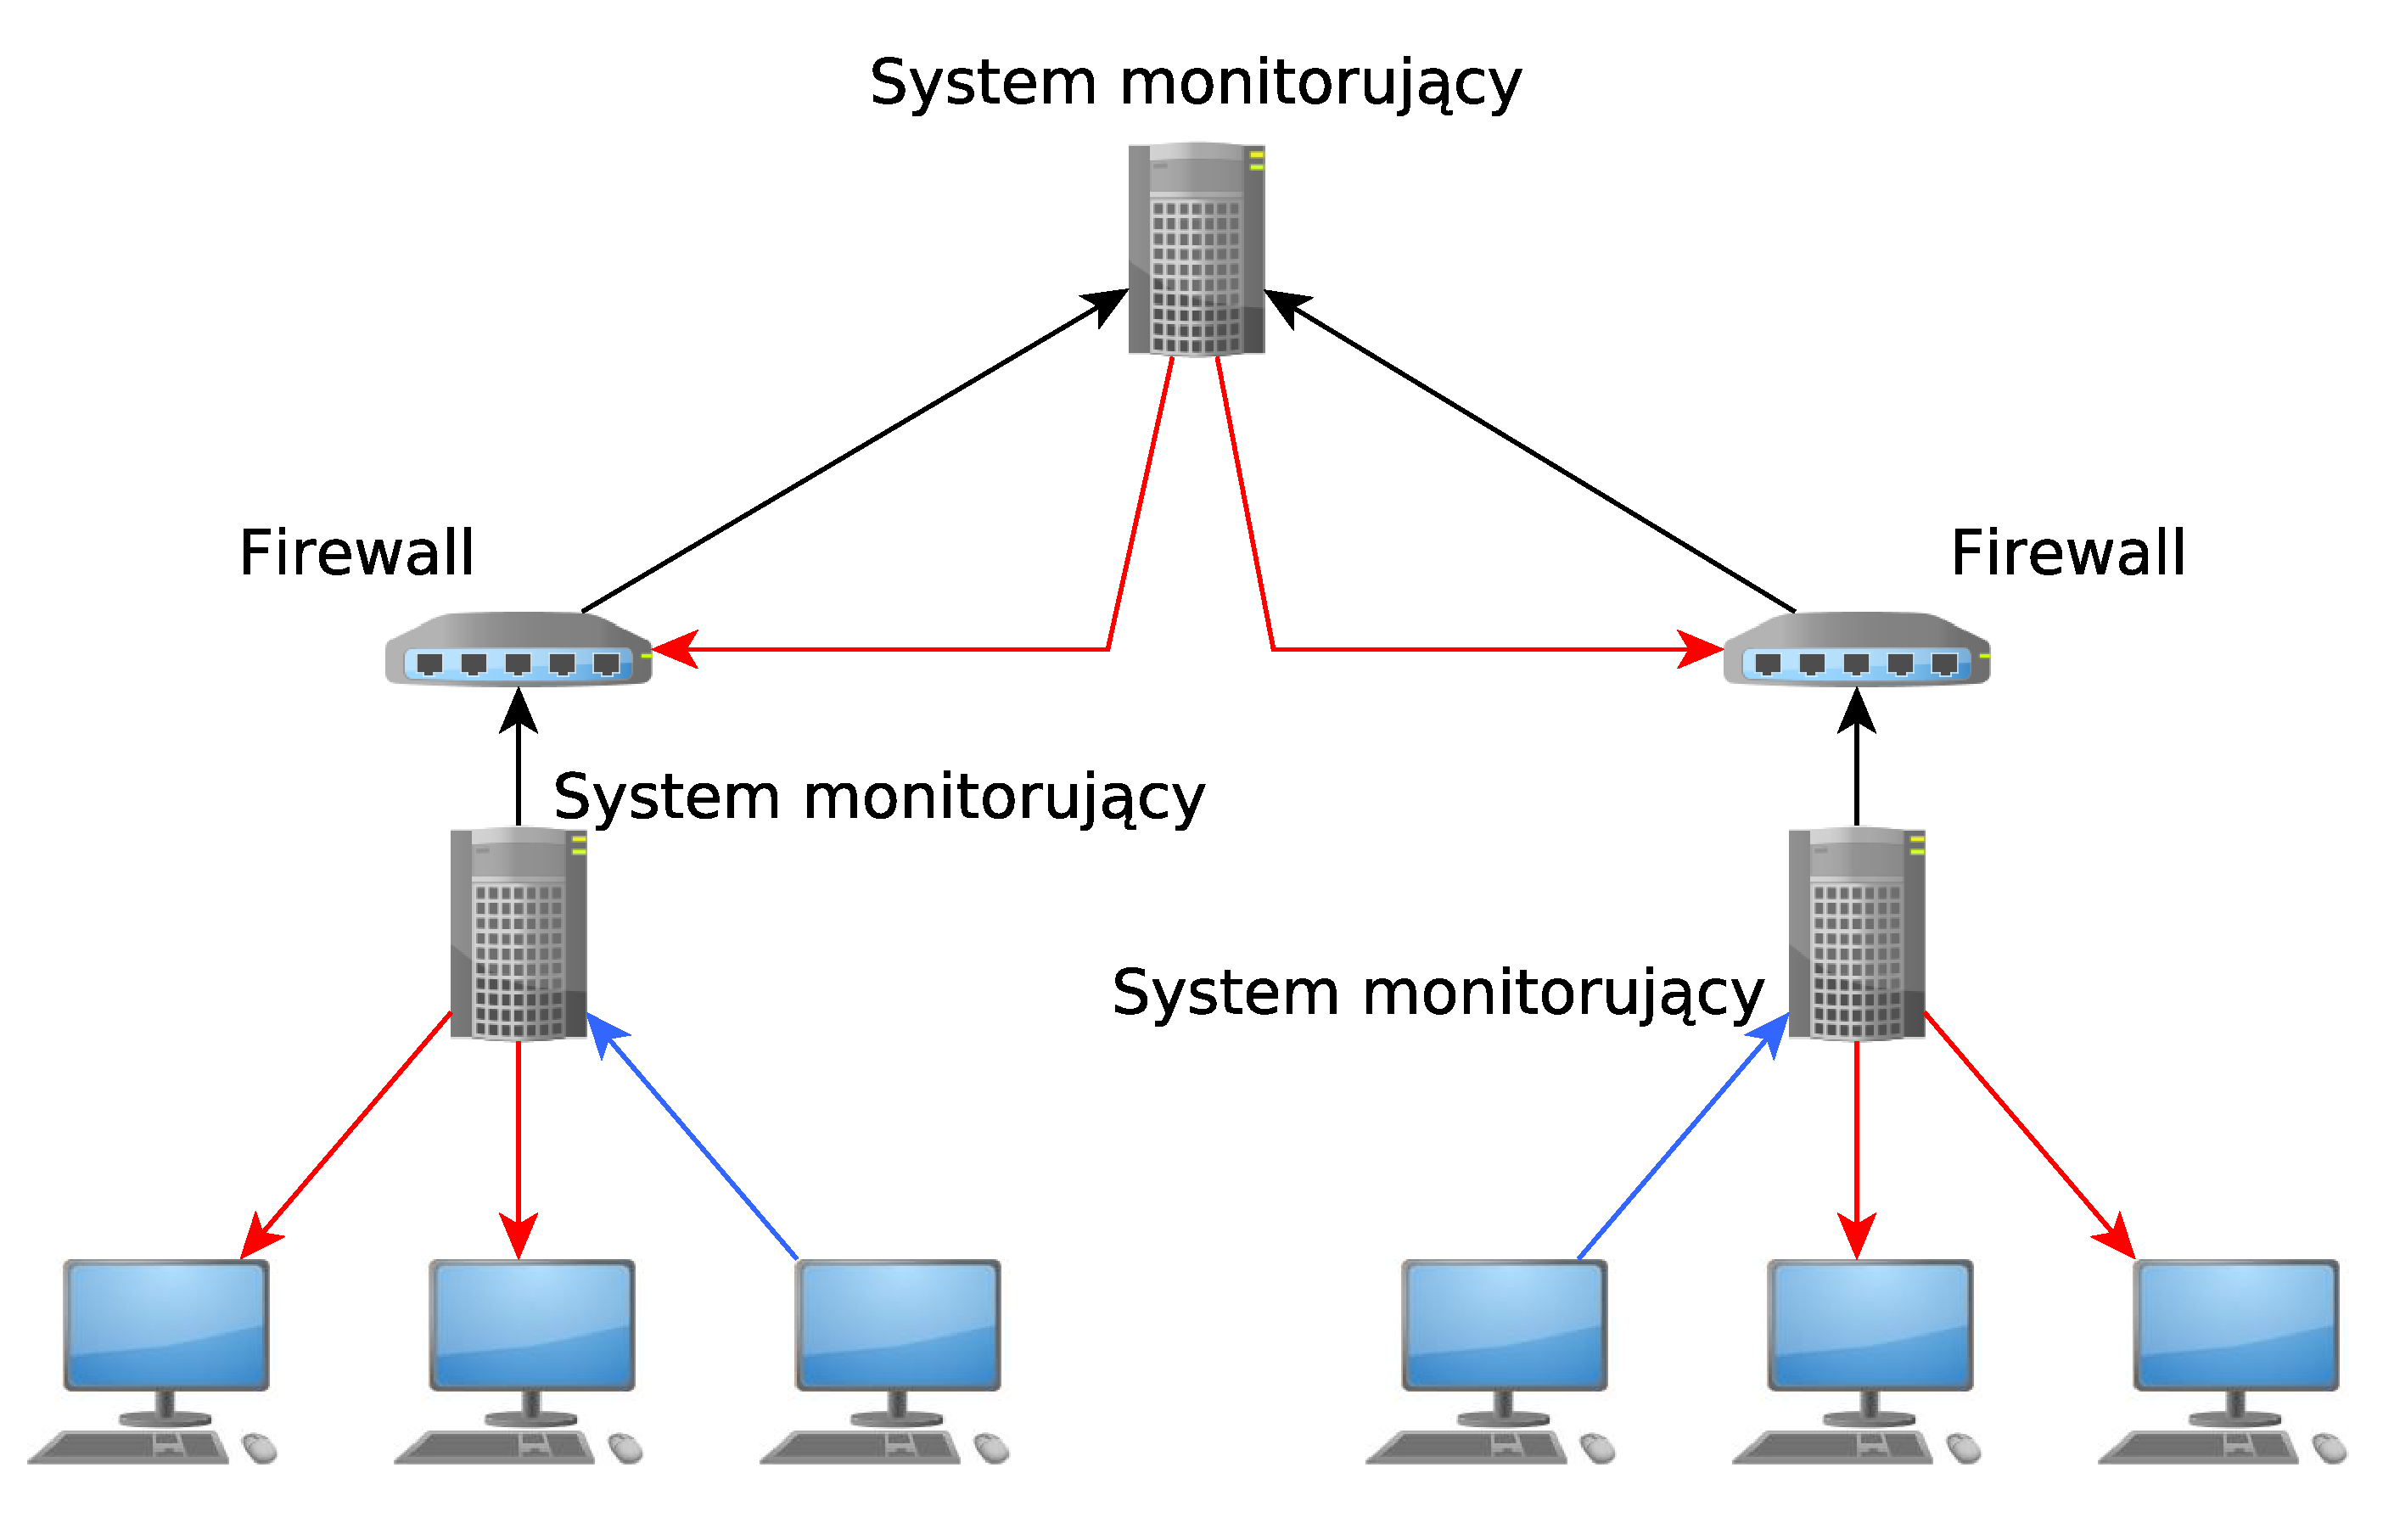
\includegraphics[width=0.49\textwidth]{img/rozproszone}
}\\[0.1cm]
\end{figure}

Wizualizację obu konfiguracji podstawowych przedstawiono
na~\ref{fig:PorPasIRozp}. Użycie monitorowania pasywnego dla
wszystkich usług jest bardzo nie wygodnie i~jednocześnie utrudnia
konfiguracje, a~także pozbawia administratora możliwosci używania
niektórych mechanizmów dostępnych wyłącznie dla urządzeń
monitorowanych aktywnie. Ponadto wyniki sprawdzeń pasywnych nie są
akumulowane, lecz wysyłane odrazu po ich uzyskaniu. Oznacza to, że
jeśli pojawi się chwilowy brak połączenia z~serwerem, to wpisy
dziennika zostaną zgubione. W~przypadku, gdy jedynym celem systemu
jest monitorowanie dostępności danej usługi zewnętrznej serwera, a~nie
jego parametrów wewnętrznych jest to jednak błąd pomijalny. Błąd ten
staje się jednak istotny, gdy jednym z~zadań systemu, jest gromadzenie
i~analiza danych historycznych. Wieloinstancyjny system minitorujący
wymaga zdecydowanie więcej zasobów jednak pozwala na osiągnięcie
znacznie wygodniejszego i~bardziej niezawodnego systemu. Ponadto
dzięki takiej konfiguracji nie ma potrzeby ingerencji w monitorowane
serwery co redukuje ich obciążenie, a~także zwiększa
bezpieczeństwo. Warto również wspomnieć, że na przykład system Icinga,
daje możliwość integracji wielu instancji jądra monitorującego, przy
pomocy wspólnej bazy danych. Dzięki temu administrator danej sieci ma
możliwość monitorowania i kofigurowania wielu instancji przy pomocy
wspólnego interfejsu. Niestety w systemie Nagios rozwiązanie to
zaliczane jest do cześci korporacyjnej tego systemu, przez co posiada
zamknięte źródła i jego wykorzystanie wymaga zakupu
licencji. Rozwiązania oparte na istnieniu jednej centralnej instancji
jądra systemu monitorujacego, do której przesyłane są, gdy jest to
możliwe odczyty wykonane przez inne instancje, są zazwyczaj darmowe
lecz wymagają dodatkowej instancji, zajmującej sie agregacją
danych. Nalezy również zwrócić uwagę, iż niektóre sytemy jak Cacti nie
posiadają w~ogóle możliwosći rozproszonego monitorowania.

\section[Monitorowanie rozproszone][Monitorowanie rozproszone klientów
mobilnych]{Monitorowanie rozproszone klientów mobilnych}

Rosnąca w~ostatnich latach popularność technologii mobilnych
przyczyniła się do pojawienia się w~firmach bardzo dużej liczby
urządzeń mobilnych, które wymagają zarówno zarządzania jak
i~monitorowania. Urządzenia mobilne są używane bardzo często przez
przedstawicieli handlowych, a~także przez menadżerów w~celu
umożliwienia wykonywania pracy poza obszarem firmy. Ponadto coraz
więcej firm świadczących zaawansowane technicznie usługi wyposaża
swoich pracowników w~bardzo drogi sprzęt, który wymaga ciągłego
monitorowania. Duże korporacje coraz częściej decydują się również na
wyposażenie swoich pracowników w~smartfony lub tablety, które mają
ułatwić współpracę z~firmą w trakcie podróży służbowych czy spotkań
z~klientami.

Klient mobilny posiada szereg cech, które znacząco odróżniają go od
klientów statycznych. Przedewszystkim należy zauważyć, że urządzenia,
o~których mowa bardzo często pracują poza obszarem firmy. Wynika
z~tego iż nie zawsze możliwe jest utrzymywanie takich urządzeń
w~wirtualnej sieci prywatnej, gdyż urządzenie może znaleźć się
w~obszarze, gdzie nie ma dostępu do internetu. Ponadto nie zawsze
konieczne jest, aby urządzenia mobilne pracowały podłączone do sieci
firmowej, gdyż dla użytkownika często wymagany jest jedynie dostęp do
internetu i~inne funkcje tego urządzenia. Warto więc zauważyć, że
urządzenia te są często narażone na dostęp do sieci, o~bardzo niskim
poziomie zaufania i~wielu zagrożeniach. Oznaczia to w~szczególności,
iż urządzenie mobilne zazwyczaj posiada zmienny adres IP, który rzadko
jest adresem globalnym. Również struktura sieci, z~której korzystają
klienty mobilne jest dynamiczna i~znajduje się poza obszarem
monitorowania administratorów danego przedsiębiorstwa. Znacząca
większość klientów mobilnych dzięki kontaktom z~siecią poza firmową
posiada, w~przeciwieństwie do klientów statycznych, możliwość
synchronizacji swojego czasu czy to z~serwerami czasu światowego, czy
też z~sieci GSM.

Należy również zwrócić uwagę na duże rozproszenie klientów
mobilnych. W~przeciwieństwie do klientów statycznych, którzy zazwyczaj
pracują w~pewnych grupach lub fragmentach sieci, klienty mobilne są
zazwyczaj rozpatrywane pojedyńczo. Większość klientów mobilnych
operuje w~pełni samodzielnie, zatem liczność grupy klientów
wynosi~1. Powoduje to, że w przeciwieństwie do klientów statycznych
gdzie grup koniecznych do wydzielenia było zazwyczaj kilka lub
kilkanaście, w~przypadku klientów mobilnych takich grup może być
kilkaset lub nawet kilka tysięcy. Warto również dostrzec różnice
w~zasilaniu. Klienty mobilne zazwyczaj posiadają własne zasilanie,
przez co każda operacja wykonywana na nim nie tylko spowalnia jego
działanie, lecz również zmniejsza jego czas pracy pomiędzy
ładowaniami. Przenośność klienta mobilnego zmienia również jego
stopień bezpieczeństwa. Urządzenia mobilne stosunkowo często są
gubione lub kradzione, co nie było możliwe w~przypadku klientów
statycznych. W~związku z~możliwością utraty urządzenia, nie powinno
sie na nim przechowywać tajnych danych, dzięki którym możnaby
skompromitować cały system z~którego korzysta klient.

Klient mobilny znacznie różni się swoją charakterystyką od klienta
statycznego. Różni się również rodzaj monitorowanych
usług. W~przypadku klientów statycznych znaczna część wysiłków jest
ukierunkowana na pomiar usług świadczonych przez dany system na rzecz
innych systemów. Natomiast w~przypadku klientów mobilnych istotniejsze
wydaje się być monitorowanie parametrów wewnętrznych danego klienta.

\section[Wymagania][Wymagania systemu monitorowania klientów
mobilnych]{Wymagania systemu monitorowania klientów mobilnych}

Klient mobilny posiada zdecydowanie odmienną charakterystykę niż
klient statyczny. Dokonano zatem analizy, jakie wymagania należy
spełnić, aby dostarczyć system, który sprosta oczekiwaniom
administratów urządzeń mobilnych jak i statycznych.

Odbiorcą systemu mają być duże firmy i~korporacje, które posiadają
bardzo rozbudowaną sieć wewnątrz firmy, a~ponadto udostępniają swoim
pracownikom urządzenia mobilne różnej klasy. Wsród tych urządzeń
znajdują się przedewszystkim telefony oraz tablety z~systemem
operacyjnym Android oraz Windows Phone, a~także liczne laptopy
wyposażone w system Windows lub Linux. Konieczne jest zatem, aby
system pozwalał na monitorowanie każdej z~wspomnianych platform. Duże
firmy oraz korporacje, zazwyczaj posiadają już oprogramowanie służące
do minitorowania swojej infrastruktury sieciowej. Aby umożliwić
administratorom łatwe zarządzanie oraz monitorowanie zarówno klientami
mobilnymi jak i~statycznymi, należy zapewnić integrację systemów
monitorowania obu kategorii klientów. Dane odczytywane na urządzeniu
mobilnym mogą zawierać zarówno dane prywatne pracownika, jak
i~tajemnice handlowe firmy. Oba te rodzaje danych nalezą do kategorii
poufnych i~powiny być należycie chronione. Ponieważ urządzenie mobilne
będzie pracowało często poza siecią firmową, podczas tworzenia systemu
należy zwrócić szczególną uwagę na kwestię bezpieczeństwa przesyłanych
danych. Ponieważ system, musi przesyłać dane poprzez sieć publiczną,
konieczne jest również zapewnienie odporności systemu na ataki
zewnętrzne oraz na próby przekazywania sfałszowanych danych do
systemu. Wszystkie wymagania stawiane przed omawianym systemem zostały
zebrane w \ref{tab:Wymagania}.

\begin{longtable}[c]{|c||p{3.5cm}|p{9cm}|}
\caption{Wymagania systemu monitorowania klienta mobilnego} \label{tab:Wymagania} \\ 
  \hline
  Kod & \multicolumn{1}{c|}{Nazwa} & \multicolumn{1}{c|}{Opis} \tabularnewline
  \hline \hline
  \endfirsthead

  \multicolumn{3}{c}%
  {{\tablename\ \thetable{} -- Kontynuacja z~poprzedniej strony}} \\
  \hline
  Kod & \multicolumn{1}{c|}{Nazwa} & \multicolumn{1}{c|}{Opis} \tabularnewline
  \hline \hline
  \endhead

  \hline \multicolumn{3}{|r|}{{Kontynuacja na następnej stronie}} \\ \hline
  \endfoot

  \hline\hline
  \endlastfoot
  
  W1 & \raggedright{Spójność danych} & \raggedright{System musi zapewnić, że wpisy dziennika nie zostaną zgubione. System musi zapewniać spójność danych pomiędzy serwerem, a~klientem mobilnym.} \tabularnewline
  \hline

  W2 & Integralności & \raggedright{System musi zapewnić, że wpisy dziennika dostarczone do serwera nie zostały w~żaden sposób zmodyfikowane lub dodane.} \tabularnewline
  \hline

  W3 & Autentyczność & \raggedright{System musi zapewnić, że odebrane dane pochodzą od uprawionego klienta.} \tabularnewline
  \hline
  
  W4 & Poufność & \raggedright{System musi zapewniać poufność danych przesyłanych od klienta poprzez szyfrowanie.} \tabularnewline
  \hline

  W5 & \raggedright{Dodawanie algorytmów} & \raggedright{System musi być niezależny od algorytmu kryptograficznego stosowanego podczas przesyłania danych. Ponadto system musi umożliwać dodawanie w prosty sposób nowych algorytmów kryptograficznych.} \tabularnewline
  \hline

  W6 & \raggedright{Uwierzytelnienie klienta} & \raggedright{System musi zapewnić możliwość uwierzytelnienia klienta.} \tabularnewline
  \hline

  W7 & \raggedright{Wymienne algorytmy uwierzytelnienia klienta} & \raggedright{System musi być niezależny od algorytmu uwierzytelnienia kliena. Ponadto system musi umożliwaić dodanie w prosty sposób nowych algorytmów uwierzytelnienia klienta.} \tabularnewline
  \hline

  W8 & \raggedright{Uwierzytelnienie serwera} & \raggedright{System musi zapewniać, iż wpisy dziennika zostaną przesłane tylko do wyznaczonego, uprawnionego serwera.} \tabularnewline
  \hline

  W9 & \raggedright{Odporność na zgubienie urządzenia} & \raggedright{Systes musi być odporny na zgubienie urządzenie. Oznacza to iż zgubienie urządzenia nie może powodować kompromitacji całego systemu.} \tabularnewline
  \hline

  W10 & \raggedright{Dostarczanie w wiele miejsc} & \raggedright{System musi umożliwiać przekazywanie danych do wielu podsystemów monitorujących, bez konieczności ich retransmisjii z~klienta mobilnego.} \tabularnewline
  \hline

  W11 & \raggedright{Reguły definiowane dla każdego klienta} & \raggedright{System musi umożliwiać definowanie reguł dotyczących miejsc przeznaczenia dla każdego klienta indywidualnie.} \tabularnewline
  \hline

  W12 & \raggedright{Oszczędność pasma} & \raggedright{System powinien minimalizować ilość przesyłanych danych. Ponadto powinien skrócić do minimum czas oczekiwania na potwierdzenie przetworzenia przesłanych danych.} \tabularnewline
  \hline

  W13 & \raggedright{Integracja z~istniejącymi systemami} & \raggedright{System monitoringu klienta mobilnego musi mieć możliwość integracji i~współpracy z~istniejącymi systemami monitorowania klienta statycznego.} \tabularnewline
  \hline

  W14 & \raggedright{Analiza danych bierzących} & \raggedright{System musi umożliwiać prezentację oraz analizę danych bierzących, a~także posiadać możliwość reagowania na wystąpienie zdefiniowanych przez użytkownika zdarzeń.} \tabularnewline
  \hline

  W15 & \raggedright{Analiza danych historycznych} & \raggedright{System musi umożliwiać analizę zadanych danych historycznych włączając w~to ich graficzną reprezentację.} \tabularnewline
  \hline

  W16 & \raggedright{Kontrola danych wejściowych} & \raggedright{System musi prowadzić kontrolę danych wejściowych od klientów. Konieczne jest aby system umożliwiał definiowanie jakie dane mogą być dostarczane przez jakich klientów.} \tabularnewline
  \hline

  W17 & \raggedright{Łatwość dodawania nowych sprawdzeń} & \raggedright{System musi umożliwiać dodawanie w łatwy sposób możliwości monitorowania nowych usług i~parametrów.} \tabularnewline
  \hline

  W18 & \raggedright{Klient dla platformy Android} & \raggedright{System musi udostępniać klienta pozwalającego na monitorowanie urządzeń opartych na platformie Android} \tabularnewline
  \hline

  W19 & \raggedright{Klient dla platformy Windows Phone} & \raggedright{System musi udostępniać klienta pozwalającego na monitorowanie urządzeń opartych na platformie Windows Phone} \tabularnewline 
  \hline

  W20 & \raggedright{Klient dla platformy Windows 8} & \raggedright{System musi udostępniać klienta pozwalającego na monitorowanie urządzeń opartych na platformie Windows 8} \tabularnewline
  \hline

  W21 & \raggedright{Klient dla platformy Linux} & \raggedright{System musi udostępniać klienta pozwalającego na monitorowanie urządzeń opartych na platformie Linux} \tabularnewline
  \hline
\end{longtable}

\section[Decyzje projektowe][Podstawowe decyzje projektowe]{Podstawowe decyzje projektowe}

Przedstawione wymagania pozwalają na opracowanie systemu, który
zaspokoi potrzebę monitorowania klienta mobilngo. System monitorujący
stanowi duży zestaw programów wykonujacych się na różnych urządzeniach
i~w~różnych kontekstach. Zaprojektowanie i~implementacja od podstaw
systemu monitorującego, który spełniłby wszystkie przedstawione
wymagania, daleko wykracza, poza ograniczenia czasowe pracy
inżynierskiej. Ponadto dobre praktyki programistyczne, nakazują
możliwie szerokie wykorzystanie gotowych programów. Nalezy również
pamietać, iż każdy program wymaga testowania i~późniejszego utrzymania
jego kodu. Wykorzystanie gotowego systemu, pozwala na uzyskanie niskim
nakładem czasu systemu, który został już dokładnie przetestowany,
a~utrzymanie jego kodu zapewniane jest poprzez osoby zewnętrzne.

W~związku z~powyższym w~niniejszej pracy podjęto decyzję, aby budowany
system monitoringu klienta statycznego był oparty o jeden z dostępnych
darmowych systemów monitorowania. Na podstawie analizy systemów
monitorujacych dostępnych na rynku, dokonanej w~\ref{chap:Systemy},
został wybrany system monitorujący Icinga.

Wybór ten podyktowany jest wieloma zaletami tego systemu. Przede
wszystkim, nalezy zauważyć przemyślaną architekturę. Ponieważ posiada
on budowę modularną, możliwe jest jego instalowanie na wielu odrębnych
urządzeniach co znacząco moze przyśpieszyc analizę danych. Możliwe
jest również monitorowanie infrastruktury w~sposób rozproszony. System
ten umożliwia zarówno monitorowanie pasywne, jak
i~wieloinstancyjne. Należy również wyróżnić system Icinga, gdyż jako
jedyny udostępnia on w~sposób darmowy, możliwość wspólnego zarządzania
i~podglądu wieloinstancyjnego systemu monitorującego. Nowoczesny
i~dynamiczny interfejs użytkownika dostarczany przez ten system, może
być w łatwy sposób rozszerzany o~dodatkowe funkcjonalności. Na
szczególne uznanie zasługuje również rozbudowana i~na bieżąco
aktualizowana dokumentacja projektu. Najważniejszą z~zalet jest jednak
popularność tego systemu wśród administratorów. Dowodem popularności
i~wiarygodności systemu Icinga może być jego zastosowanie w~ośrodku
badań Europejskiej Organizacji Badań Jądrowych CERN\footnote{Szerszy
  opis zastosowania systemu Icinga w tej organizacji można znaleźć
  w~\cite{www:IcingaCern}.}.

Rdzeń monitorujący systemu Icinga jest przeznaczony dla systemu Linux,
jednak możliwe jest uruchomienie go na większości systemów z~rodziny
Unix. W~związku z~powyższym wszelkie rozwiązania zaimplementowane
w~ramach tej pracy, są przeznaczone, dla tych samych systemów co
jądro monitorujące.
